\title{ PyEDA: \\ A Software to analyze Normal Modes in NMR and MD Structures using an Essential Dynamics approach.\thanks{ Introduction to Pythons $\&$ Structural Bioinformatics - M. Sc. in Bioinformatics for Health Sciences at Universitat Pompeu Fabra}}
\author{Joan Francesc Gilabert  $\&$ David Mas  - Prof:Javi Garcia $\&$ Baldo Oliva. }
\date{\today}

\documentclass[12pt]{article}
\usepackage{amsfonts}
\usepackage{amssymb}
\usepackage{amsthm}
\newtheorem{theorem}{Theorem}
\usepackage{mathtools}
\usepackage{enumerate}
\usepackage[a4paper, margin=2.5cm]{geometry}
\usepackage{tikz}
%\usepackage{tikz}
\usetikzlibrary{decorations.markings,arrows}
\usepackage{pgfkeys}
\usepackage{natbib}
\bibliographystyle{nature}
\usepackage{graphicx}
\usepackage{listings}
\usepackage{xcolor}
\lstset{basicstyle=\footnotesize,
  showstringspaces=false,
  commentstyle=\color{orange},
  keywordstyle=\color{blue},
  stringstyle=\color{purple}
}
\usepackage{subfig}

\begin{document}
\maketitle

\begin{abstract}
In this project we have developed PyEDA a python based software capable to analyze Normal Modes from NMR and MD structures in pdb format. It uses a Essential Dynamics approach and it gives different outputs like a structure pdb file with the superimposed structures, the eigenvalues in decreasing order, the fluctuations of the structure by residue and a final structure with the main motions of defined normal modes applied. It can be used as a python Package,  with a tkinter interface and also as a CLI standalone program. The main dependencies of the software are BioPython\citep{Cock2009}, Tkinter, Matplotlib\citep{Hunter2007}, NumPy and SciPy\citep{VanderWalt2011} packages.
\end{abstract}

\tableofcontents


\section{Introduction to NMA and Essential Dynamics}
Normal mode analysis or NMA are powerful  and common methods used by the protein field to study the collective motions of biomolecules. Its arise comes from the fact that protein function, protein structure and protein dynamics are closely related. The way a part of a protein is moving can help us determine weather a specific part of the structure is relevant in terms of functionality. Although it is not covered in this software, dynamics analysis can also help in the use of homology modeling to  order to determine evolutionary patterns in highly conserved sequences. 

There are 3 important approaches to perform a NMA. 
\begin{enumerate} [i]
\item Standard Normal Mode Analysis
\item Elastic Network Models
\item Essential Dynamics
\end{enumerate}
The presented software uses a Essential Dynamics approach but this tutorial is going to give a brief explanation of the basics of the other approaches.\citep{Hayward2008}
\subsection{Standard Normal Mode Analysis}
The Normal Mode Analysis are mostly used to probe large-scale and shape-changing motions in biological molecules. It has connections with experimental techniques such as infrared and Raman spectroscopy but its main use is to theoretically predict motion in proteins. 

The most important Normal Modes are the ones that have greater fluctuation and lower frequency because as any other biological sequence they have emerged from evolutionary design rather than by chance. For example, a movement of a protein produced by chance will be not just in one direction but in many and therefore its fluctuation in one directory will be reduced by the fluctuation in the other directory. The movement of the protein to bind or interact with another protein will be seen in NMA as a unique Normal Mode with a great fluctuation.

In its purest form, NMA is a harmonic analysis and at the end it uses the same force fields that the ones used in the Molecular Dynamics Simulation. There are 3 steps in order to perform a NMA of a protein. 
\begin{enumerate} [i]
\item In the first step a standard NMA minimize the conformational potential energy as a function of the atomic coordinates
\item Next, it will compute a Hessian Matrix using second derivatives of the potential energy for each coordinate
\item Finally, it will compute the diagonalization of the Hessian matrix obtaining eigenvalues and eigenvectors also named as "normal modes".
\end{enumerate}
Each of these steps are very computationally demanding. Because of this complexity associated to these computations other more simple approaches have been used in order to minimize the computational cost of a NMA.

\subsection{Elastic Network Models}
The Elastic Network\citep{Tirion1996} approach is a big simplification of the problem and the results are not much different from the standard NMA considering the difference from an sNMA to reality. At the end this Elastic Network approach uses a protein model is dramatically simplified. In this model the atoms are connected by a network of elastic connections. The advantages versus the traditional approach are the elimination of the energy minimization step and the reduced number of atoms considered. The first advantage is held because the approach already consider the elastic connections to be at their minimum length. The reduced number of atoms is due to the use of $C_{\alpha}$ only for the analysis as they are the points connected in the protein. For most of the functional movements and dynamics of proteins it is enough to consider these atoms as they represent the structure shape.\citep{Hayward2008}

\subsection{Essential Dynamics}
The Essential Dynamics approach\citep{Amadei1993} is a completely different computation. It is based on a principal components analysis (PCA). This radical change have its importance in the complexity of biomolecules. Proteins and in general all of the biomolecular systems have complex dynamics simulations that can be hard to analyze and to uncover functional mechanisms or motions. This disadvantage of the previous approaches is solved using Essential Dynamics as it only remark the most important modes.  Interestingly, it has been found that most of protein dynamics can be described by a low number of degrees of freedom. Moreover this approach have the huge advantage that the dynamics can be inspected mode by mode and separately. Allowing  to use only the most characteristic modes. 

In contrast to NMA, PCA of a molecular dynamics simulation trajectory does not rest on the assumption of a harmonic potential. In fact, PCA can be used to study the degree of anharmonicity in the molecular dynamics of a simulated system. It was shown in proteins that in physiological temperatures especially the major modes are dominated by anharmonic fluctuation and therefore can be predicted using this approach\citep{Amadei1993}. 

Using Essential Dynamics, the modes are sorted according to variance rather than frequency. Nevertheless, the largest-amplitude modes of a PCA usually also represent the slowest dynamical transitions. Therefore the conclusions of an standard NMA analysis stands with this approach.\citep{Hayward2008}
\subsubsection{Steps in a Essential Dynamics approach}
The steps to perform this approach are the following:
\begin{enumerate} [i]
\item Superposition to a common reference structure. This step is crucial particularly in NMR structures.
\item Construction of a variance–covariance matrix of positional fluctuations using atom coordinates
\item Diagonalitzation of the matrix to obtain eigenvalues and eigenvectores representing the modes of motion
\item Projection of the original configurations onto a defined set of principal components to get principal coordinates. 
\end{enumerate}
The matrix construction is the key step. It is build first constructing a vector with all the 3 coordinates for each atom and for each model and then computing the means of each position for different models (for NMR structures) or time frames (for Molecular Dynamics).  After these 2 small steps the $C$ matrix is constructed as a co-variance matrix using the following equation,
\begin{equation}
C=<(x_{i}(k) - <x_{i}>) \cdot (x_{j}(k) - <x_{j}>)>
\end{equation}
where $x_{i}(k)$ and $x_{j}(k)$ are the atomic coordinates of the atoms $i$ and $j$ in
configuration $k$\citep{Amadei1993,Gargallo2003}. 

In order to obtain the modes a diagonalization step for solving this must be held.
\begin{equation}
\Lambda = \mathbb{V}^{T} \mathbb{C} \mathbb{V}
\end{equation}
where $\Lambda$ is a diagonal matrix (contining the eigenvalues) and where $\mathbb{V}$ is the matrix formed by the eigenvectors, each one corresponding to the eigenvalues of $\Lambda$.

The eigenvectors are the representation of each normal mode. The eigenvalue that is associated with a eigenvector (or mode) indicates the relative contribution of that mode (or eigenvector) to the motion of the whole protein structure.\citep{Gargallo2003}

Therefore, the normal modes can be sorted using the eigenvalues as representation of their contribution to the protein. Usually in decreasing order. For a structure of N atoms, $\mathbb{C}$ would be a 3N × 3N matrix. As a result of the diagonalitzation, $3N − 6$ eigenvectors with nonzero eigenvalues will be obtained. There should be 6 eigenvalues equal to 0 because the corresponding eigenvectors describe the overall rotation and translation that is eliminated in the superposition step. In practice, with full-protein structures and considering $M$ as the number of models or frames, we will get most of the times $M-1$ eigenvalues different from $0$ because most of the times $3N > M$ this conditions will be true. To sum up, in most of the analyses we would be able to obtain $M-1$ nonzero eigenvalues which is not a big deal considering we are only interested in the major ones\citep{Hayward2008}. 

The next step is the projection of the principal component into principal coordinates. To do so, the following 2 equations have been used:
\begin{equation}
p_{i}(k)=\mu_{i}\cdot (x(k) - <x>) 
\end{equation}
\begin{equation}
x'_{i}(k)=p_{i}(k) \cdot \mu_{i} + <x>
\end{equation}
In equation 3 we project the eigenvectors to the original coordinates to get the principal coordinates or $p_{i}$ and then, in equation 4 we transform back these projections to Cartesian coordinates. This is an important step for visualization of the motions. In equation 3, the eigenvector is represented with the $\mu$ and the particular coordinate is represented with $x(k)$. In Equation 4, the representation stands.\citep{Hayward2008}
\clearpage
\section{Practical Tutorial}
\subsection{Work-flow}
The workflow is summarized in the following figure:

\vspace{1cm}
\begin{figure}[h]
\centering
\includegraphics[scale=0.45]{DyagramFlow_NMA}
\caption{Entire Workflow for EDA}
\label{fig:workflow}
\end{figure}
As seen in the figure \ref{fig:workflow}, the user can introduce either a file or a pdb code. If the user introduce a pdb code the software retrieve the structure from pdb (if internet connection is available). The structure that must contain Models or Frames in order to analyze the Normal modes. Then the Superimposition takes place and generates the first pdb file with the superimposed strucutres of the different modes. After that the Essential Dynamics step is performed obtaining the eigenvectors and eigenvalues that represent the normal modes. The regular plots obtained after this step (eigenvalues vs eigenvector index) can be obtain through a matplotlib integration in a Tkinter window. After that, the projection is performed and the projections plots (RMSD vs Residue Number) is sent to the same Tkinter window mentioned before. The final step is to generate a final pdb file containing the projected structure.

As you can see the main dependencies are included in the figure and represented by their logos when used. The Tkinter interface covers almost all steps from loading the data to the software to the plots in the visualization step. Moreover, BioPython\citep{Cock2009} and NumPy and SciPy\citep{VanderWalt2011} packages are used almost everywhere. This Software is based in a \textit{"do not reinvent the wheel"} approach. The generated pdb files can be visualized using either CHIMERA or PyMol softwares. 

\subsection{Step by Step guide}
\subsubsection{Checking Dependencies}
Before stariting the installation procedure we have to check whether or not we have the required packages installed. Open a shell terminal windows and enter into the python3 console. Type the following to see if the packages are installed.
\begin{lstlisting}[language=Python]
$ python3
>>> import numpy
>>> numpy.version.version
'1.10.2'
>>> import scipy
>>> scipy.version.version
'0.17.0'
>>> import tkinter
>>> tkinter.TkVersion
8.5
>>> tkinter.TclVersion
8.5
>>> import Bio.PDB
>>> import Bio
>>> print(Bio.__version__)
1.66
\end{lstlisting}
Note that it may work with older versions, these versions are the ones used to build the software. If some of this imports do not import the package you must installed before using our software. 
\subsubsection{Installing the Package}



\subsubsection{Usage}
\paragraph{CLI Usage}
 \paragraph{Graphical Usage}
 The graphical usage is set by default. You only need to call the software via terminal like this. 
\begin{lstlisting}
 $ python3 -m PyEDA
 \end{lstlisting}
 
 We have experienced some troubles depending on the OS used in the PDBio class. In some cases the superimposed file "pdbcodealign.pdb" is saved with extra "END" lines that do not let the user directly see the pdb structure in PyMol. If it is your case, we provide ypu here a fast awk one-liner to solve the problem. 
 \begin{lstlisting}
 $ awk '$0 ! ~ /^END$/ {print $0} END {print "END"}' 1msfalign.pdb > corrected.pdb
 \end{lstlisting}
\section{Analysis of the performance and results}
\subsection{Comparison of the results with Van Aalten 1998}
In order to test the performance of our software we have used the analysis done by Van Aalten et al 1998 \citep{VanAalten1998} of a NMR structure of the Myb DNA-Binding Domain. We have been able to reproduce 2 important figures of the article. 
In the article, they have used an Essential Dynamics approach to analyze the Normal Modes of the NMR structure Mouse c-Myb R2R3 [PDB entry 1MSF\citep{Ogata1994}]. They have found large fluctuations of atoms that describe a hinge-bending motion between R2 and R3 repeats. They have observed that only with NMR data. After that, the authors have also used a Molecular Dynamics Simulation to predict and quantify the motion. Finally they have tested the effect of a proline to alanine mutation into the motion observed. The motion in the mutated protein was found to be enhanced. 

The 1MSF structure is a NMR file with 25 Models of a binding protein to the a DNA chain. In the figure \ref{fig:1MSF_super} we can see the first output of PyEDA, a superimposed structure of all the structural modes using PyMol\citep{PyMOL}. 

\begin{figure} [h]
\centering
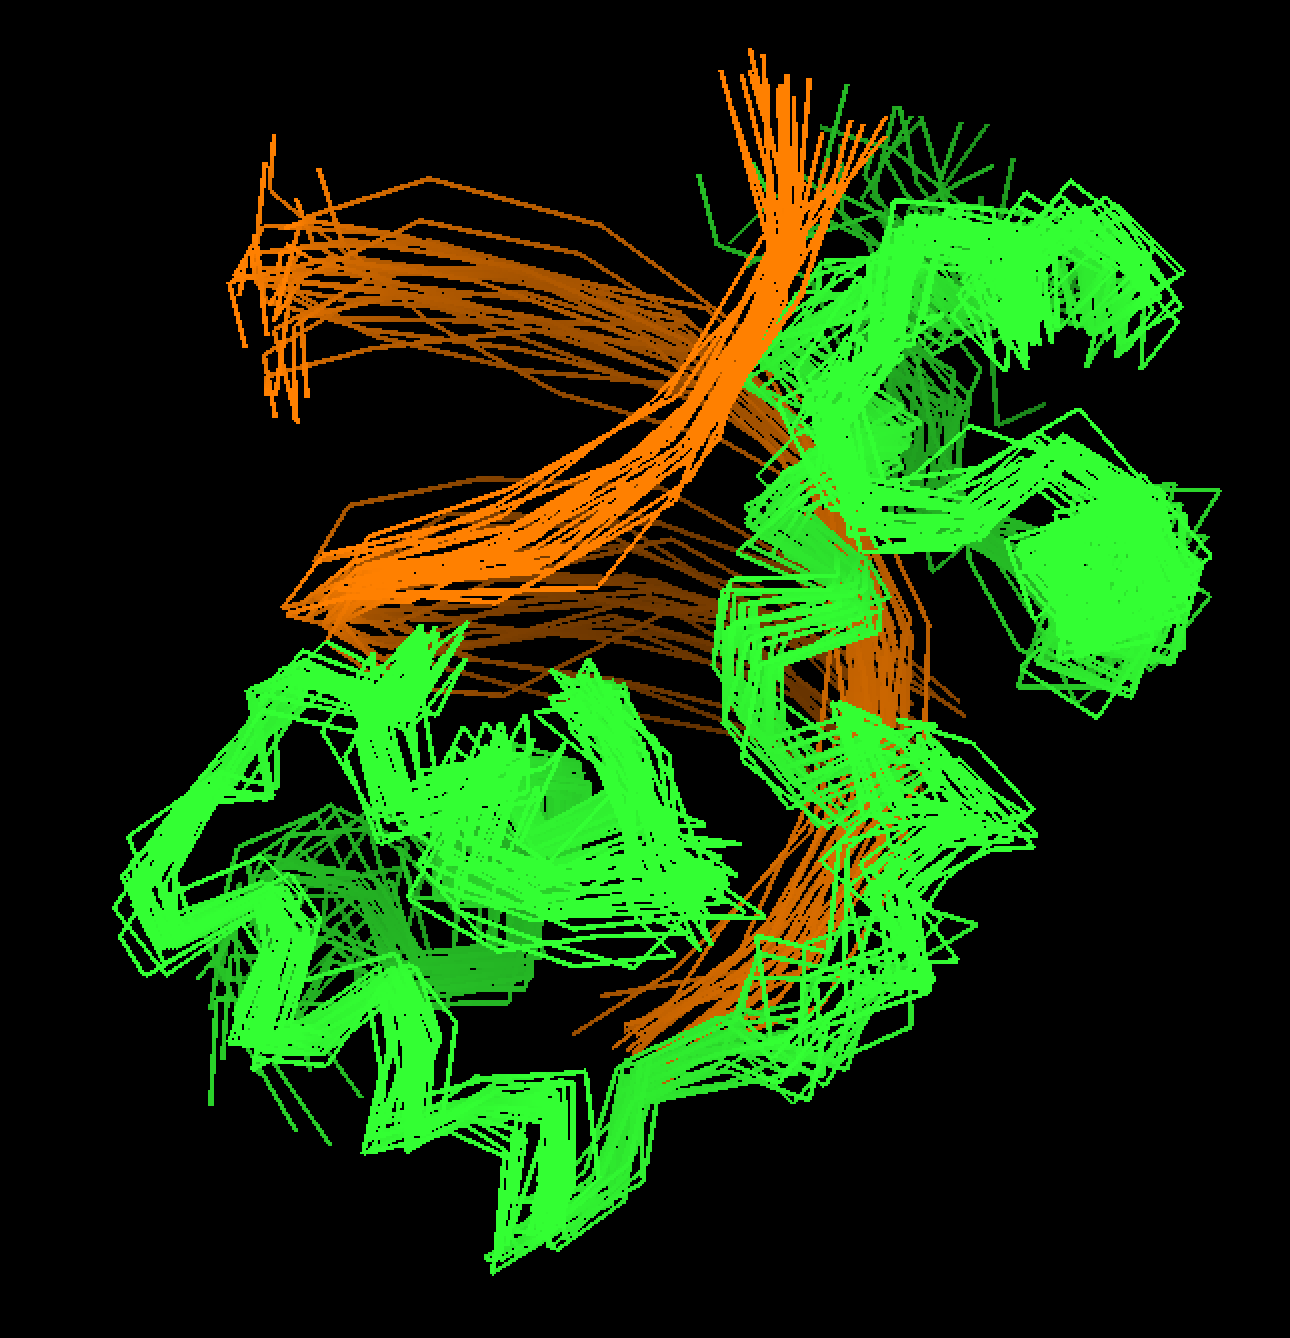
\includegraphics[scale=0.4]{pymol_1mSF}
\caption{1MSF superimposed structure}
\label{fig:1MSF_super}
\end{figure}
Although this structure in particular is already superimposed in the pdb file we can see clearly how the different models are here superimposed. To check the superimposition capacity we have used a non superimposed pdb file(see subsection 3.2). 

\begin{figure} [h]
\centering
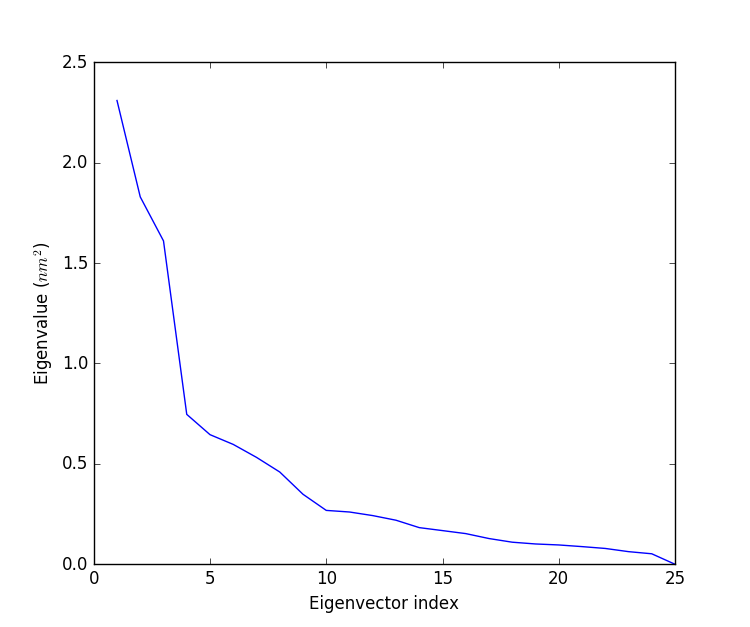
\includegraphics[scale=0.6]{1MSF_figure}
\caption{Eigenvalues against their corresponding eigenvector indexes}
\label{fig:1MSF_figure}
\end{figure}


In the following output of the program, figure \ref{fig:1MSF_figure}, we can see each eigenvalue of the different eigenvectors ranked by the contribution on the protein motion. The contribution is measured with the eigenvalue of each eigenvector. Here we can see the 24 eigenvectors expected considering that there where 25 models in the initial pdb file. This plots give us an idea of how each eigenvector is influencing the protein motion. The shape of the plot is identical to the literature \citep{VanAalten1998} so we can assume that the performance of the software is optimal. We can see how the most important part of the movement is kept by the first 5 or 10 eigenvectors. This is a typical behavior for proteins and it give us the capability to distinguish between the evolutionary fixed moves and the random ones. Although this plot is important to understand the system, biologically it gives us information that in fact there is a evolutionary conserved move.  

\begin{figure} [t]
\centering
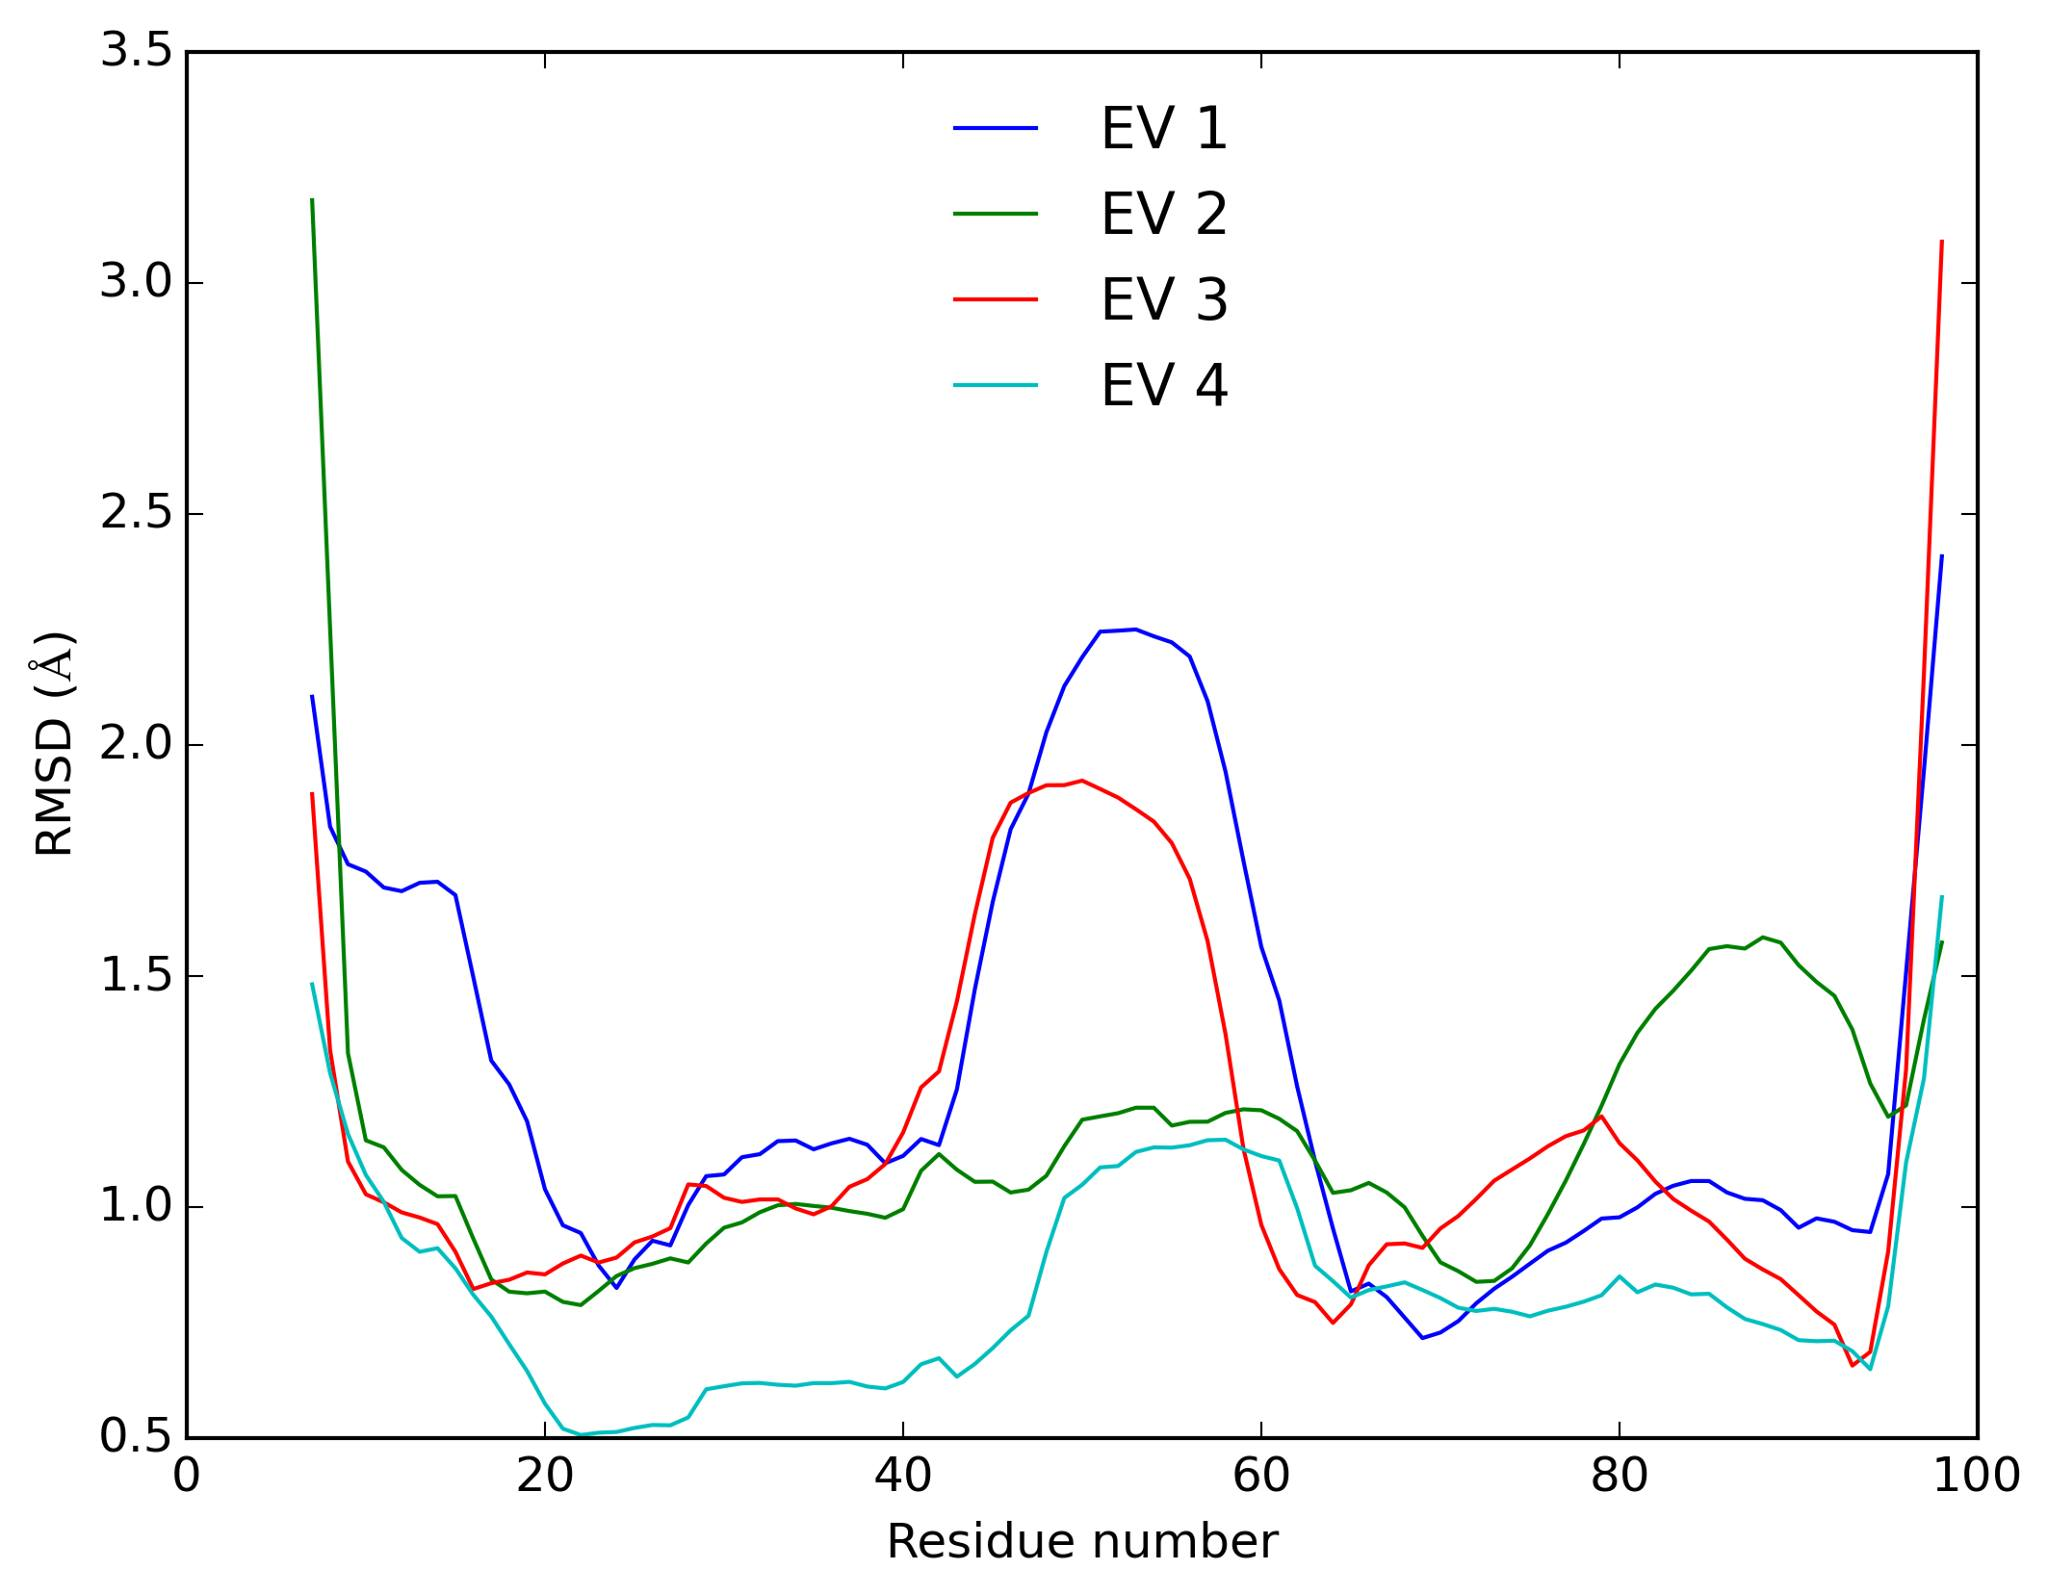
\includegraphics[width=0.75\textwidth]{Normal_Modes_residue}
\caption{After the projections were computed for each eigenvector, the two structures with the minimum and maximum projections along that eigenvector were used for the superposition. The window size used are 15aa.}
\label{fig:1MSF_residue}
\end{figure}

\begin{figure} [t]
\centering
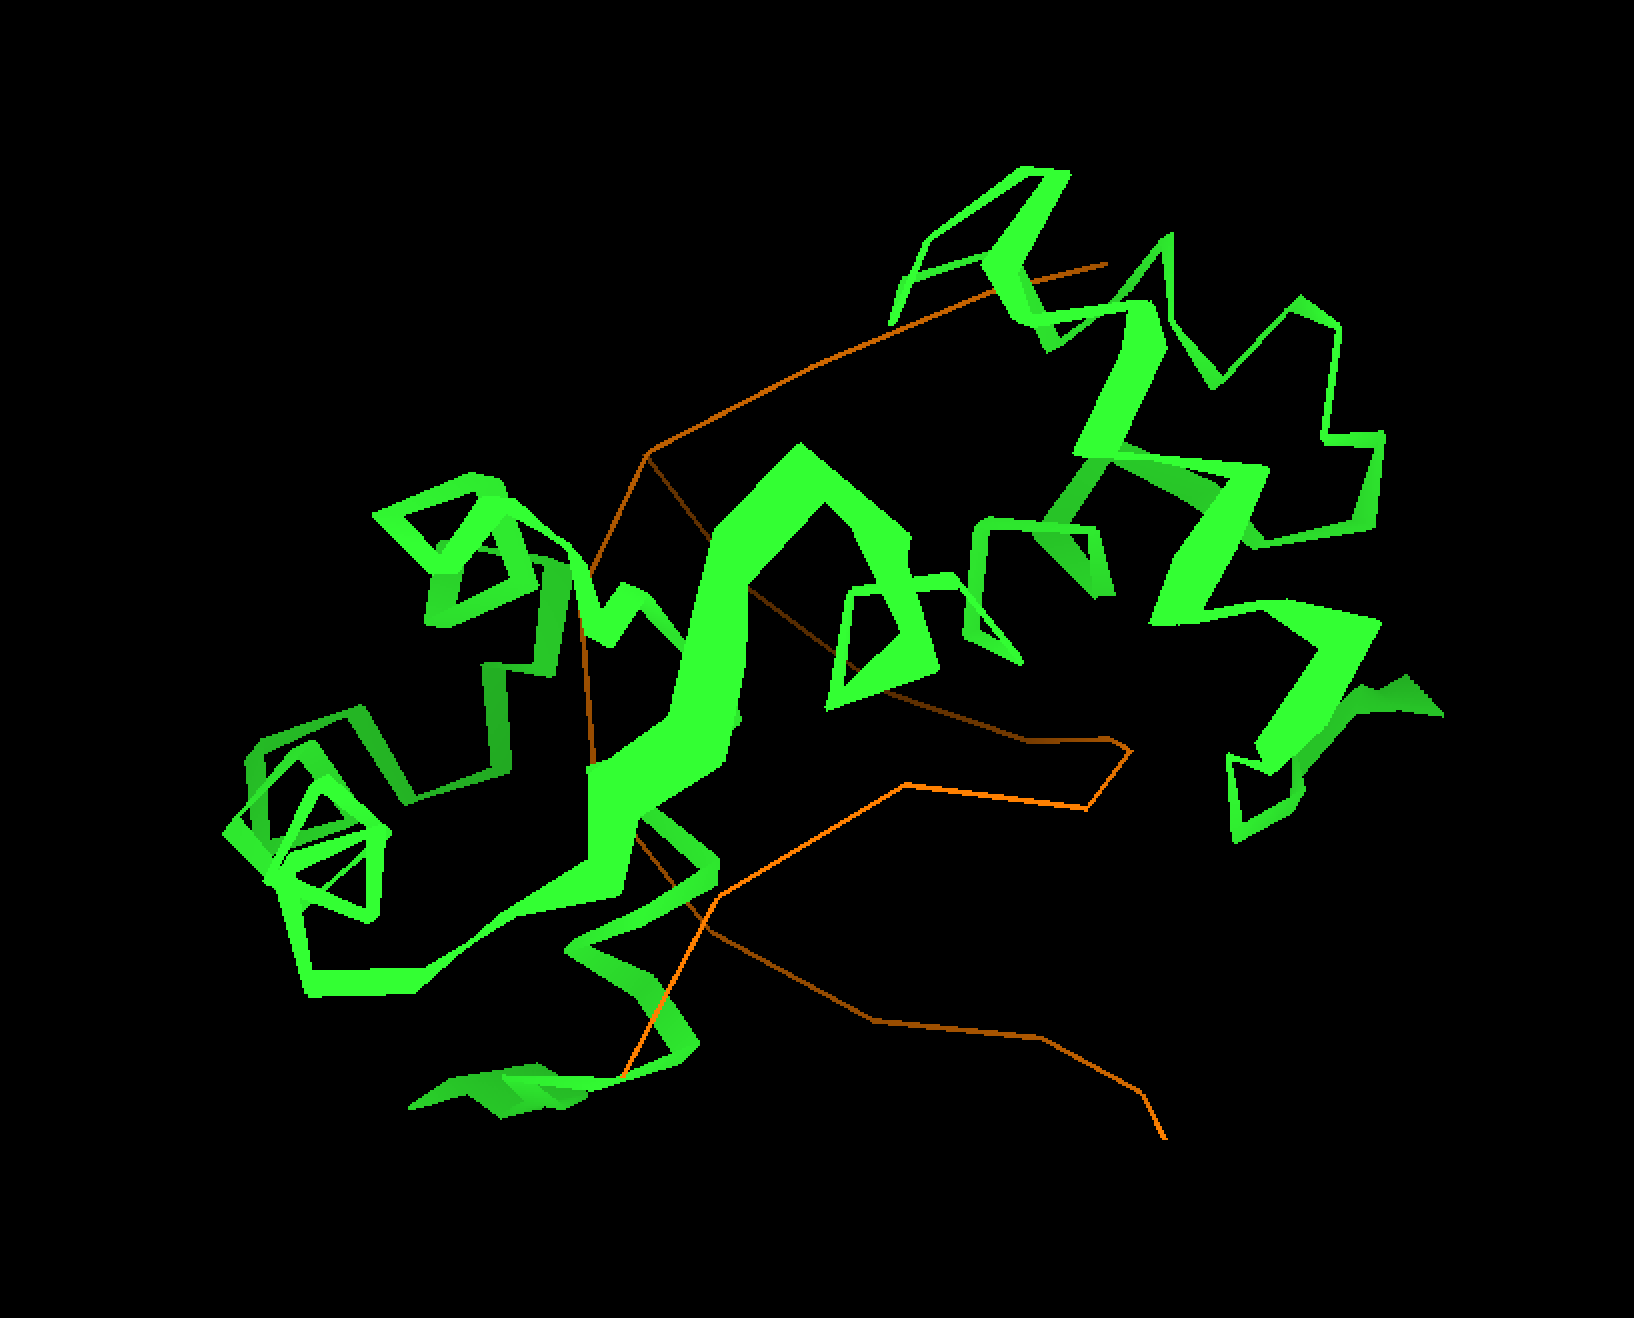
\includegraphics[width=0.75\textwidth]{1msf_allstates}
\label{fig:1msf_all}
\caption{Projected models from 1MSF with total full-span of 3 and step of 0.1 using the first eigenvector}
\end{figure}


The net step of the program is to project the original structure with the trajectory of a given vector. Therefore we can see the different structures generated by applying that eigenvector. In order to quantify this motions of the protein the most diferent 2 structures from the ones projected are superimposed in sliding-window fashion with an window value of 15 residues. For each window a root mean sqare deviation (RMSD) of all $C_{\alpha}$ positions is computed. This can be seen in the figure \ref{fig:1MSF_residue} that is also almost identical to the literature figure\citep{VanAalten1998}. This type of plot gives us important biological information and the ability to quantify the observed movement. As the authors stress on the paper\citep{VanAalten1998} this shape shows a hinge-bending motion between residues 40 and 60 where the R2 and R3 repetitions end and start respectively. 

The final output of the Program will give us a pdb file containing the projections of a defined eigenvector to the original structure stored as different models of the structure. This file, seen in platforms like PyMol\citep{PyMOL} is useful to see the actual motion derived from the eigenvector. In this case, this projected file show clearly a hinge-bending motion as the authors state in the paper. A interesting thing to consider is that the hinge-bending motion will be only observed when considering the first and third eigenvectors. As it can be seen in \ref{fig:1MSF_residue} the other eigenvectors do not capture this motion. In the figure \ref{fig:1msf_all} we can see all the generated states in one image but the proper way to see the motion is using the PyMol commands, 
\begin{lstlisting}
 > hide everything
 > show ribbon 
 > mplay
 \end{lstlisting}
It is also possible to see how the residues between the 2 repetitions and the ens of the protein are that get most of the motion. As the motion is larger in the connection between both repetitions in the animation is easy to resemble the bending motion. 





\subsection{Testing superimposition with 1JOY structure}
In order to test the first steps of the software analysis we have used the solution structure of the homodimeric domain of Envz protein from Escherichia coli [PDB entry 1JOY\citep{Tomomori1999}]. This structure is also a NMR and as can be see in figure \ref{fig:1joy_notsuper} the database pdbfile is not superimposed.  

\begin{figure}[h]
  \centering
  \subfloat[1joy from pdb]{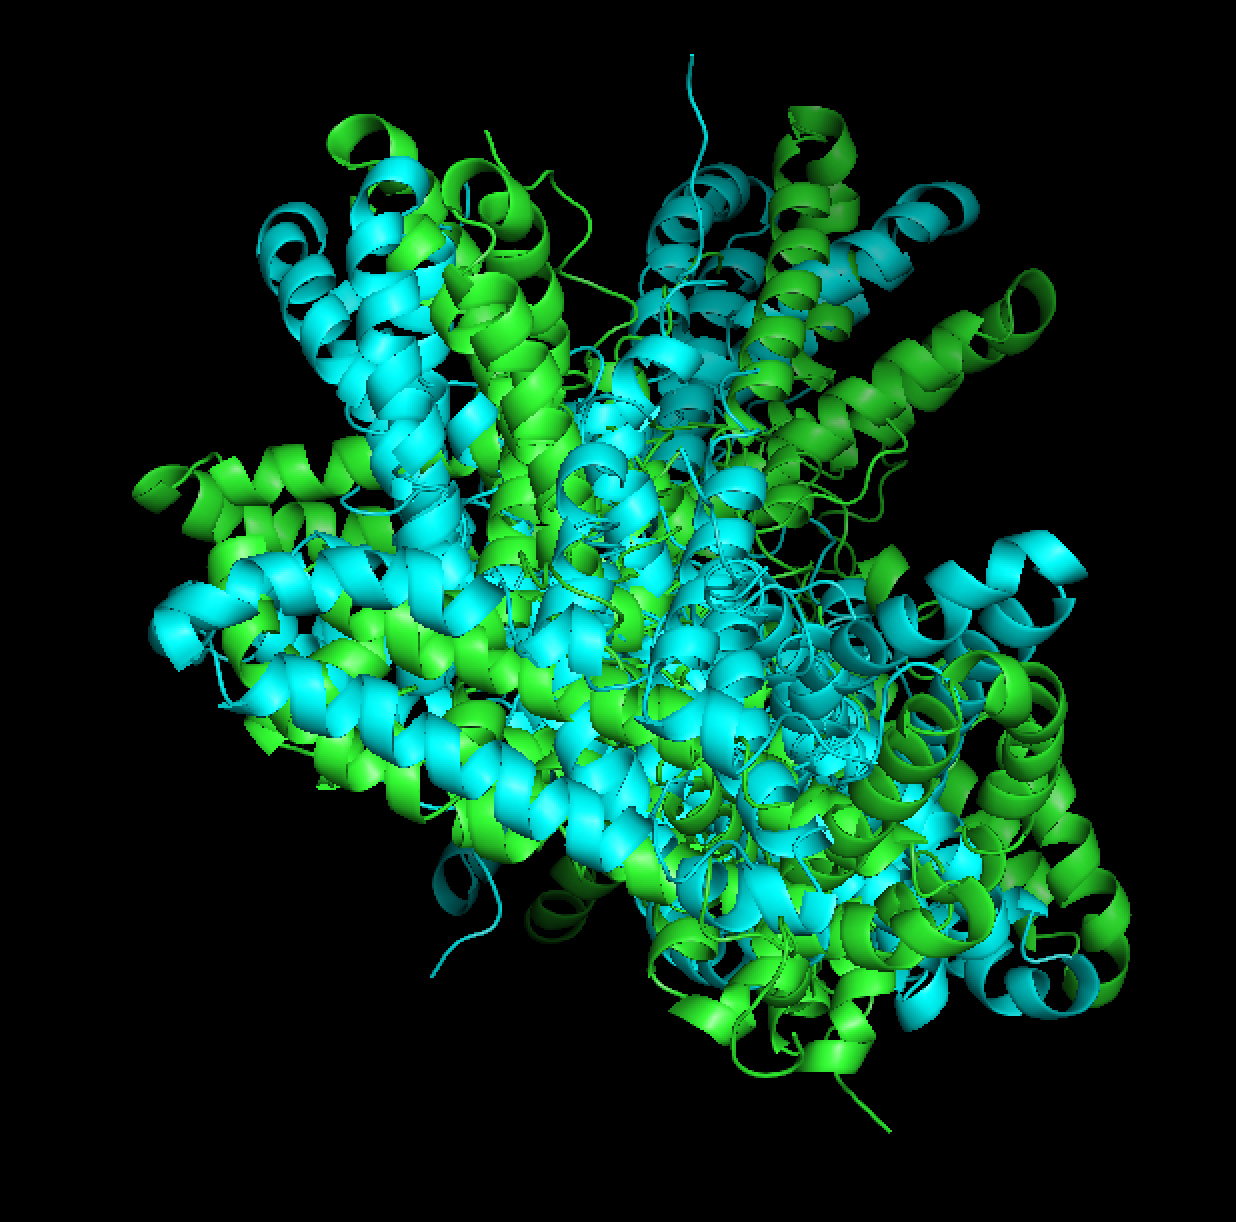
\includegraphics[width=0.475\textwidth]{1joy_pdb}\label{fig:1joy_notsuper}}
  \hfill
  \subfloat[Superimposed 1joy]{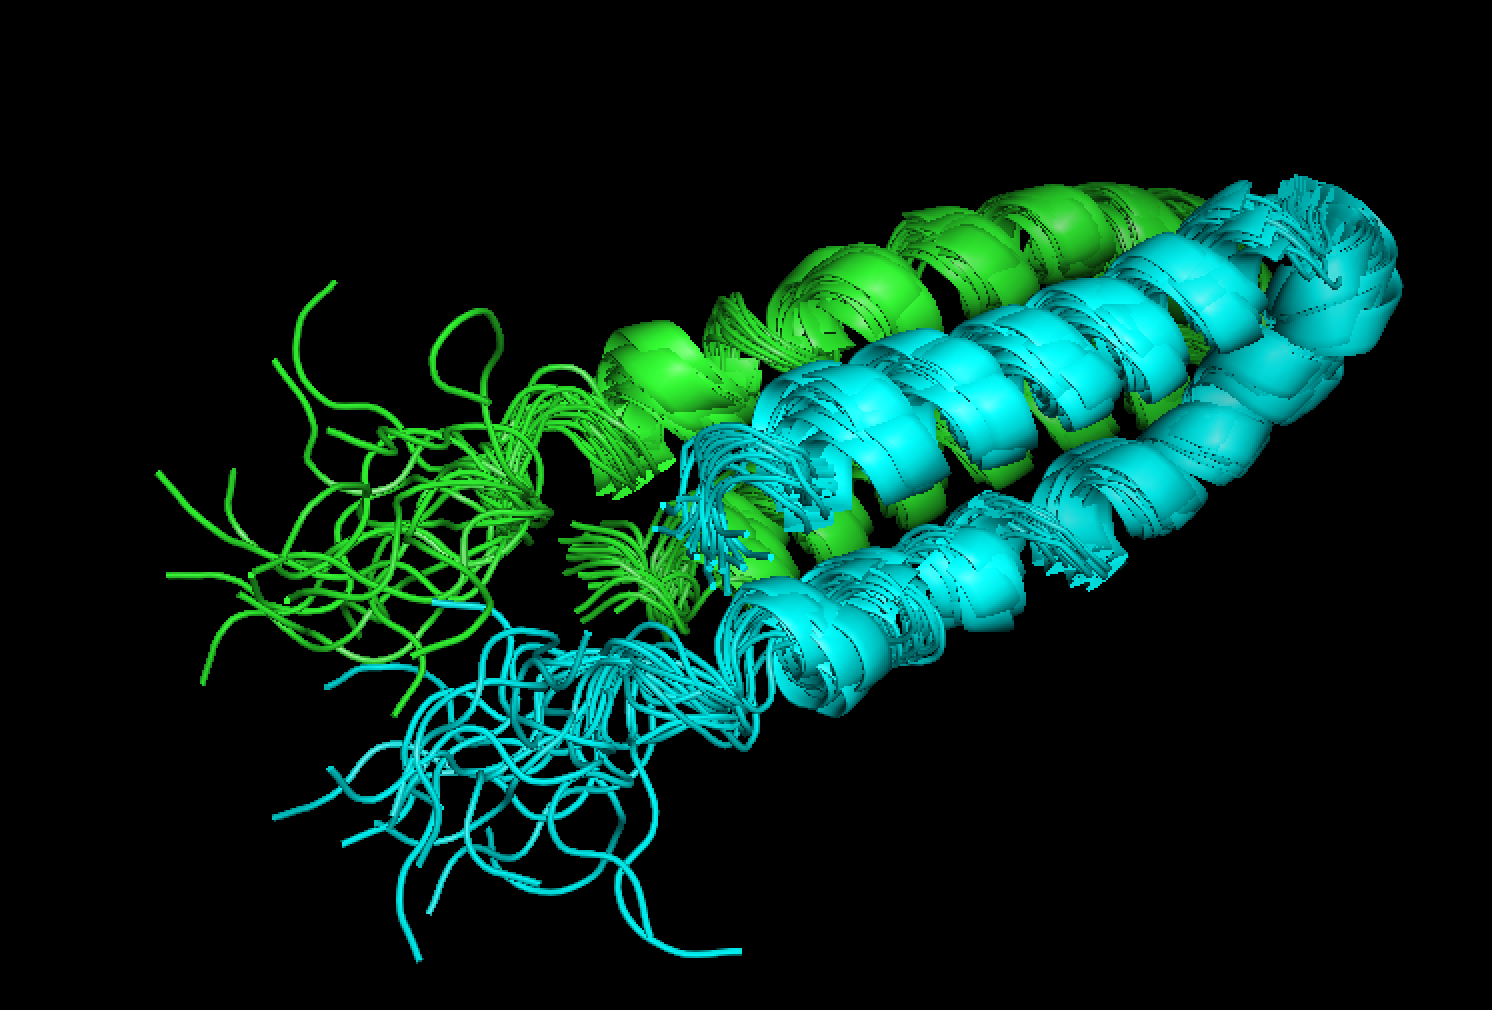
\includegraphics[width=0.475\textwidth]{1joy_super}\label{fig:1joy_super}}
  \caption{PyMol\citep{PyMOL} visualitzation of the a) original 1joy structure directly retrieved from the pdb and the b) superimposed 1joy structure by PyEDA.}
\end{figure}

The superimposition is a critical step in our software, without one of this steps the actual protein movement could not be observed. The figure  shows at the left panel the pdb original file and in the right panel the superimposition done by our software. It is quite clear the change between the 2 images and it is useful in terms of considering the importance of this step. Although the RMSD values are not a output of our software the image show how the superimposition strategy is optimal. 

This structure is usefull to see how protein with more than one chain can be also analyzed. This protein have a homodimeric structure formed by a 60 residues long  chain. The motion of this NMR structure is localized on the N-terminal end which is bigger than the C-teminal end. As predicted, in the figure \ref{fig:1joy_residue} we can see big fluctuation at the first residues and after the 60th residue that indicates the end of the first chain. 

\begin{figure} [!h]
\centering
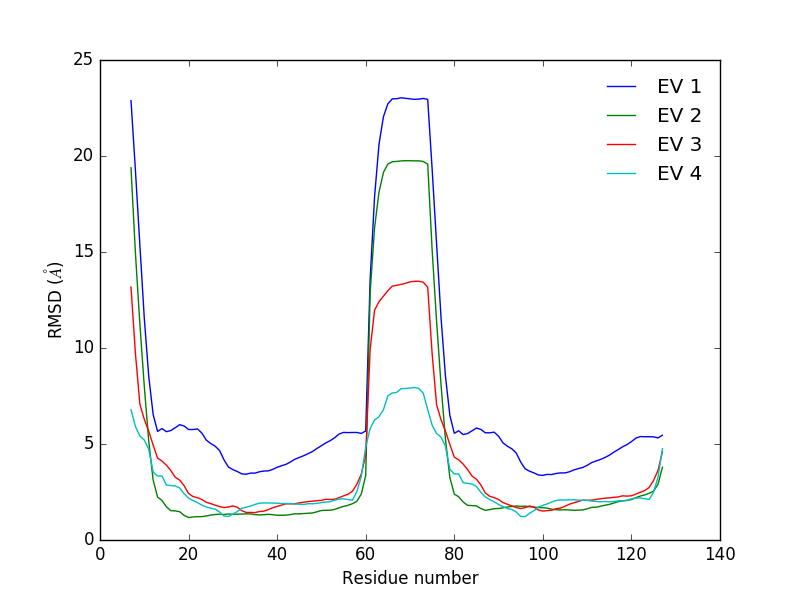
\includegraphics[width=0.8\textwidth]{1joy_residue}
\caption{Plot of the most different projected structures. Window size used, 15aa.}
\label{fig:1joy_residue}
\end{figure}
\subsection{Conclusions and Caveats}
PyEDA is a wrap up of the Essential Dynamics approach to get a Normal Mode Analysis of any NMR pdb structure and any MD pdb-like file. As conclusion we may stress that PyEDA is a promising and useful tool specially for the analysis of protein dynamics.  It is a unified and complete analysis tool to get protein motion. It is designed to easily uncover and quantify the functional motions of NMR and MD structures. It can be used autonomously using the guided graphical interface or using the CLI which gives the user the possibility to automatize the process. It also have a easy and user-friendly installation process and it is based on the most used programming language, python. 

The main improvement that we could implement in the future is a PyMol integration to the tkinter graphical interface. This feature have not been implemented because the actual version of PyMol have only a python2.7 integration meanwhile PyEDA is based on python3. Although a patch code exist to use PyMol with python3 we believe that it may be a stable version of the program in order to distribute PyEDA with the appropriate PyMol integration. 

As a major caveats we must stress the large number of dependencies PyEDA have and a previously mentioned problem with the "END" keyword in the pdb file writting that we have not been able to find the source. PyEDA have dependencies on  BioPython\citep{Cock2009}, Tkinter, Matplotlib\citep{Hunter2007}, NumPy and SciPy\citep{VanderWalt2011} packages but if the user is a python experimented bioinformatician these packages should be installed and updated in their system. Moreover, to non-experimented python users these packages can also be easily installed using the pip3 module. 

The "END" bug have only been detected in a mac OS meanwhile in fedora it works perfectly. These may be because of some Biopython dependencies. It should run okay in other machines but in case the bug is happening to you we propose an awk one-liner to easily correct this error (see section 2). 

\clearpage
\listoffigures
\bibliography{Bibfile}

\end{document}